\Chapter{Menetrend-alkalmazások}

% Le kell írni, hogy milyen típusú menetrendek vannak, milyen jellegű problémák merülnek fel a menetrendi adatok nyilvántartásánál.
* Érdemes minél több hasonló alkalmazást megemlíteni, bemutatni, és össze is hasonlítani őket, ahol lehet.

% Az adatok hozzáférhetőségével, és az alkalmazások közötti adatátvitellel kapcsolatban is érdemes összeszedni pár dolgot.

Szinte mindegyik közlekedési vállalat közzéteszi az interneten a helyi menetrendi adatait. Az viszont, hogy ezt milyen formában teszik, már sokféle lehet. Vannak a felhasználók igényeit kielégítő, jól kezelhető alkalmazások, de vannak sajnos kevésbé felhasználóbarát megoldások is. Ezek közül szeretnék néhányat bemutatni.
Elsőként a szülővárosom helyi tömegközlekedésének menetrendjét említeném meg, melyet középiskolás éveim során napi szinten használtam. Az Észak-magyarországi Közlekedési Központ Zrt. által kiadott ózdi menetrendről van szó. Véleményem szerint az ÉMKK Zrt. által használt megoldás egyáltalán nem felhasználóbarát. A weboldalukon csupán \texttt{.pdf} formátumban vannak feltöltve a menetrendadatok. Annyi választási lehetőségünk van, hogy egy nagy PDF-ben az összes viszonylat menetrendjét böngésszük, vagy egy listából kiválasztva csak egy viszonylatét akarjuk megnyitni. A menetrend formátuma szintén nehezen olvasható. Egy táblázatban az adott viszonylat által érintett megállók, a menetidő és a megtett kilométer van feltüntetve. A táblázat alatt irányokra lebontva az indulási idők találhatók. Szerintem a legrosszabb megoldást itt alkalmazzák: az indulási idők előtt különböző jelek találhatók, ezek mondják meg, hogy az adott indulási idő mely napokon érvényes. Legalul egy jelmagyarázat van, amely alapján értelmezni tudjuk a fenti jeleket. Mindez megfigyelhető \aref{fig:EMKK_menetrend}. ábrán.

\begin{figure}[h!]
\centering
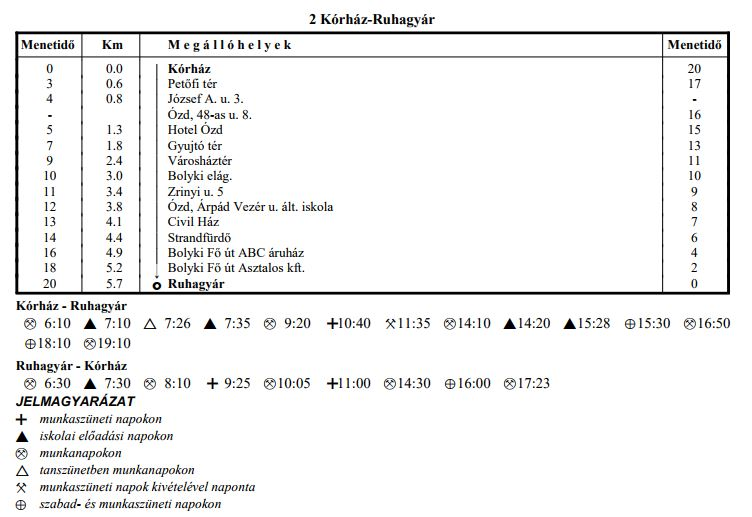
\includegraphics[scale=0.7]{kepek/EMKK_menetrend.jpg}
\caption{Egy járat menetrendje az ÉMKK Zrt. oldalán}
\label{fig:EMKK_menetrend}
\end{figure}

Szerintem ez a megoldás nagyon nehezen használható, körülményes ilyen módon megkeresni a kívánt információt.

Az útvonaltervezés nem támogatott, térképes megjelenítés van ugyan, de annak a használhatósága is erősen megkérdőjelezhető. A vonalhálózati térképet tekinthetjük meg egy képen, amin az összes járat megtalálható. Ezt ábrázolja \aref{fig:EMKK_vonalhalozat}. ábra. Szerintem nagyon átláthatatlan, sokkal használhatóbb lenne például egy Google Mapsen megjelenített változat, amelyben lehetne keresni is, és csak a kiválasztott vonalak útvonalát látni.

\begin{figure}[h!]
\centering
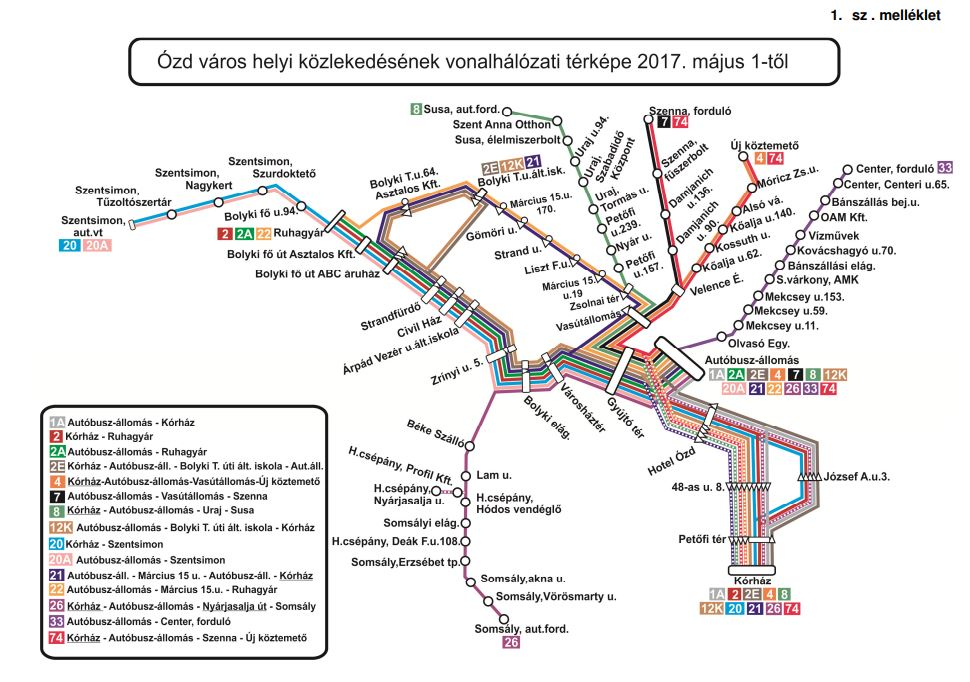
\includegraphics[scale=0.6]{kepek/EMKK_vonalhalozat.jpg}
\caption{Ózd város helyi közlekedésének vonalhálózati térképe}
\label{fig:EMKK_vonalhalozat}
\end{figure}

Másodikként a Miskolci Városi Közlekedési Zrt. weboldalán található menetrenddel és útvonaltervezéssel kapcsolatos funkciókat szeretném bemutatni. Itt is megtalálható az ÉMKK Zrt.-nél bemutatott PDF-es változat az egyes vonalakra, viszont egy jóval átláthatóbb formában. Nincsenek az indulási idők előtt különböző jelek, ehelyett három oszlopban vannak felsorolva az időpontok: munkanap, szombat, valamint vasárnap és ünnepnap szerint. A sorok pedig óránkénti felosztást valósítanak meg.

Az ÉMKK Zrt.-nél bemutatott vonalhálózati térkép fellelhető az MVK Zrt.-nél is, szerintem ez itt sem használható igazán, azonban ezek mellett sok más kényelmi funkció elérhető még az oldalukon. Lehetőség van a menetrend megtekintésére különböző szűrőfeltételek megadásával. Két oszlop jelenik meg a felületen, villamos- és autóbuszvonalakra csoportosítva a viszonylatokat. Ezt mutatja \aref{fig:MVK_menetrend}. ábra. Vonalszám, irány, megálló és egy dátum kiválasztása után a Keresés gombra kattintva megjelenik egy táblázat a megadott szűrőfeltételek eredményének megfelelő indulási időket tartalmazva. Az indulási időkre kattintva az adott járat részletes menetrendje jelenik meg, a járat által érintett megállókat, a menetidőket az adott megállókig, és a megállókból történtő indulási időket tartalmazva. A táblázat alatt Google Mapsen a járat útvonala is megjelenik.

\begin{figure}[h!]
\centering
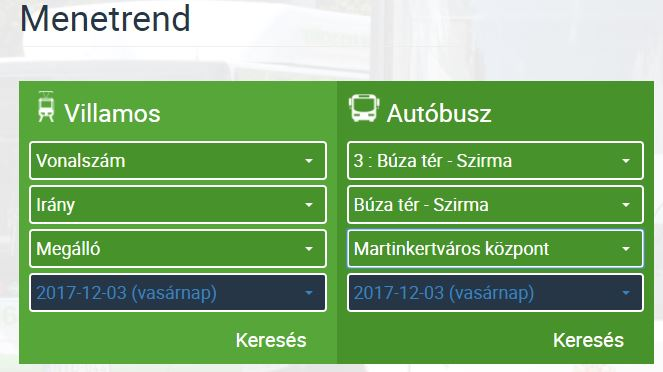
\includegraphics[scale=0.7]{kepek/MVK_menetrend.jpg}
\caption{Keresés a menetrendben az MVK Zrt. oldalán}
\label{fig:MVK_menetrend}
\end{figure}

Ezzel a felülettel kapcsolatban két észrevételem van. Észrevettem, hogy ha csak a vonalszámot választjuk ki, a többi szűrőfeltételt üresen hagyjuk, akkor a Keresés gombra kattintva automatikusan lejjebb görgetődik az oldal, ahol azonban nincs semmi, nem jelenik ilyen esetben meg a táblázat. Szerintem elegánsabb megoldás lenne, ha ilyenkor egy hibaüzenet jelenne meg, figyelmeztetve a felhasználót, hogy minden mezőt töltsön ki. A másik észrevételem a térképes megjelenítéssel kapcsolatos. Megjelenik Google Mapsen a járat útvonala, viszont túlságosan ránagyítva a kiválasztott megállóra. Véleményem szerint átláthatóbb lenne, ha távolabbról jelenítené meg az útvonalat, és a felhasználó ráközelítene, ha érdekli közelebbről egy adott szakasz.

Lehetőség van Google Maps segítségével útvonaltervezésre is, amit \aref{fig:MVK_utazastervezes}. ábra mutat. Kiválaszthatjuk, hogy honnan hova szeretnénk eljutni, megadva egy időpontot, és a Google Maps elkészíti a tömegközlekedési útvonalterveket, amelyek megjelennek a felületen.

\begin{figure}[h!]
\centering
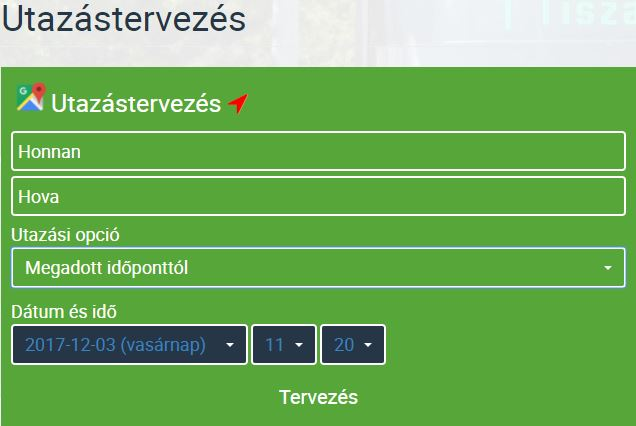
\includegraphics[scale=0.7]{kepek/MVK_utazastervezes.jpg}
\caption{Utazástervezés az MVK Zrt. oldalán}
\label{fig:MVK_utazastervezes}
\end{figure}

Összességében elmondható, hogy egy jóval több funkcióval rendelkező, használhatóbb megoldást kapunk, mint az ÉMKK Zrt. esetében.
Végezetül tekintsük át a Budapesti Közlekedési Központ Zrt. Menetrendek oldalát. Egy könnyen kezelhető, letisztult felületen lehet böngészni a menetrendet és útvonalat tervezni is. Ez látható \aref{fig:bkk_menetrend}. ábrán. A felület tetején egy gombsor található, amely segítségével a különböző típusokra szűrhetünk, mint például autóbusz, villamos, metró, hév stb.

\begin{figure}[h!]
\centering
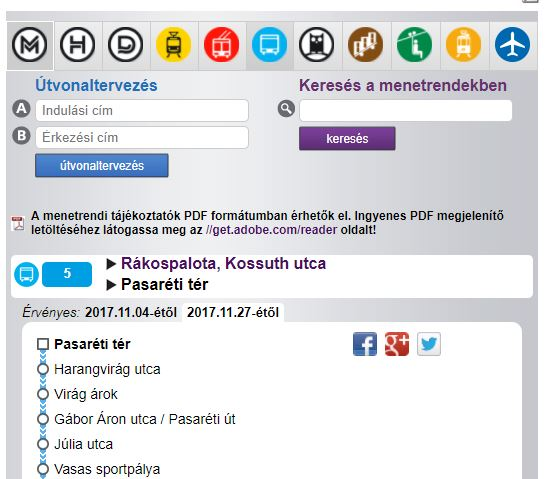
\includegraphics[scale=0.8]{kepek/bkk_menetrend.jpg}
\caption{BKK Zrt. Menetrendek}
\label{fig:bkk_menetrend}
\end{figure}

A gombsor alatt az útvonaltervezés és a keresés található. Az útvonaltervezés nagyon intelligens, nemcsak megállók neveit lehet megadni, hanem címeket és ismertebb helyeket is. Például a WestEnd, westend, west end kulcsszavak mind működtek, mindegyik esetben kicserélte a Váci út 3.-ra, ami a címe az említett bevásárlóközpontnak, és oda tervezett útvonalat. Az útvonaltervezés eredménye egy másik lapon jelenik meg, bal oldalt egy listából választhatunk több lehetséges útvonal esetén, hogy melyiket akarjuk a térképen látni, ahol a teljes útvonal látszik alapértelmezetten. Ez látható \aref{fig:bkk_terkep}. ábrán. Ezt a fajta megoldást hiányoltam az MVK Zrt. esetén.

\begin{figure}[h!]
\centering
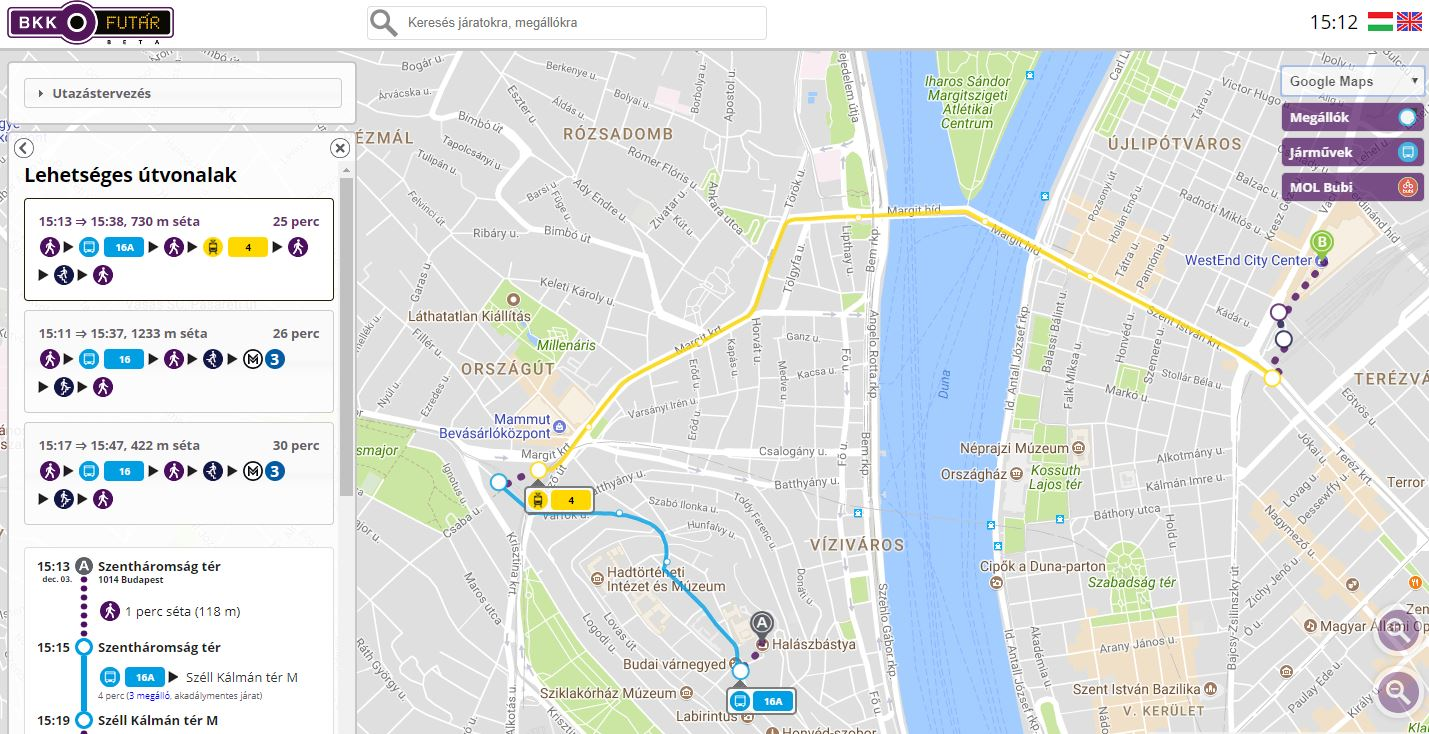
\includegraphics[scale=0.4]{kepek/bkk_terkep.jpg}
\caption{Utazástervezés a BKK Zrt. felületén}
\label{fig:bkk_terkep}
\end{figure}

Az útvonaltervezés és a keresés alatt a különböző viszonylatok listája jelenik meg, amelyekre kattintva legördül a viszonylat megállóinak a listája. A megállókra kattintva pedig egy \texttt{.pdf} töltődik be, az adott viszonylat adott megállójának menetrendjét tartalmazva.
Meglátásom szerint a három bemutatott weboldal közül ez utóbbi a leghasználhatóbb, az itt található funkciók a legfelhasználóbarátabbak.
